\chapter{Behavior Analysis Based on Fused Multimodal Data}

\section{Introduction}
Chapter 4 established entity-level correspondences across heterogeneous modalities and produced a unified representation for each physical target. This representation retains trajectory information together with modality-specific attributes, making it richer than a single-source track. However, target fusion does not by itself determine whether an entity behaves normally. In monitoring scenarios, the system must also judge whether a target follows a plausible route, whether its speed and motion shape deviate from normal patterns, and whether its behavior remains coherent with nearby targets.

This chapter studies behavior anomaly detection for the fused entities generated in Chapter 4. The setting differs from conventional trajectory anomaly detection in two respects. First, the input is an object-aligned fused entity rather than a trajectory from one sensor. Its observations may come from optical, thermal, electromagnetic, SAR, or other modalities with different visibility and sampling characteristics. Second, abnormality may appear at multiple semantic levels. A target may be individually abnormal because its route, speed, or motion shape is unusual. It may also be group-wise abnormal when it departs from the local motion pattern of neighboring targets.

This chapter asks how object-aligned multimodal fusion results can be converted into reproducible anomaly evidence at the individual, group, and situation levels. To address this question, behavior analysis is organized into an individual-level detector, a group-level detector, and a score-fusion stage that projects object-level evidence into situation-level outputs. The individual-level detector follows a route-speed-shape design. Fused trajectories are converted into route, speed, and shape feature sequences, and an LSTM autoencoder learns the normal pattern of each feature type. Reconstruction errors are then adjusted by embedding-space neighborhoods, and multiple detector outputs are fused by rank-based ensemble scoring.

\section{Related Work}

\subsection{Trajectory-Based Anomaly Detection}
Trajectory-based behavior analysis studies how motion traces reflect normal movement patterns, abnormal deviations, and high-level target activities. Early trajectory mining methods relied mainly on geometric similarity, density statistics, clustering, and local trajectory segmentation. Representative work such as TRACLUS partitions trajectories into meaningful line segments and groups similar sub-trajectories to discover common movement patterns \cite{lee2007traclus}. The partition-and-detect framework further showed that abnormal behavior may appear in a local part of a trajectory rather than across the entire track \cite{lee2008traod}. Isolation-based trajectory anomaly detection demonstrated that unusual routes can be identified by measuring how easily a trajectory can be isolated from normal movement patterns \cite{zhang2011ibat}. These classical methods provide the basic intuition for this chapter: abnormal behavior should be analyzed from the full trajectory, local motion segments, speed changes, direction shifts, and route-level deviations.

With the development of deep representation learning, trajectory anomaly detection has moved from manually designed distances toward learned normal-pattern modeling. Recent studies attempt to model more complex trajectory distributions and richer abnormality types. CETrajAD explicitly decomposes trajectory anomalies into route, speed, and shape aspects and combines complementary detectors for different anomaly types \cite{cao2025cetrajectory}. DiffTAD introduces diffusion-based denoising for vehicle trajectory anomaly detection, treating anomaly detection as the reconstruction of a normal trajectory distribution from corrupted observations \cite{li2024difftad}. Context-aware trajectory anomaly detection further argues that coordinates alone are insufficient, and incorporates agent identity and geographic context into the reconstruction process \cite{hu2024contexttrajad}. More recently, graph-enhanced trajectory anomaly detection integrates movement-network topology, segment semantics, historical transition patterns, and confidence-weighted anomaly scoring \cite{mbuya2025getad}. These studies indicate that modern trajectory behavior analysis increasingly combines motion features, contextual semantics, and structural constraints.

The above work is highly relevant to the present thesis, but most existing methods still assume that the input trajectory is produced by a single observation source or by a relatively fixed movement network. In contrast, the behavior analysis problem considered here uses the fused entity representation generated in Chapter 4. Each entity contains both a trajectory component and modality-specific attributes. The behavior representation in this chapter therefore preserves useful motion descriptors from classical trajectory analysis while carrying forward multimodal information from the upstream fusion stage.

\subsection{Graph-Based Group Anomaly Detection}
Individual trajectory features are insufficient when the behavior of a target is constrained by surrounding targets. Early multi-agent trajectory models already recognized this issue. Social LSTM introduced social pooling to aggregate neighboring pedestrian information for trajectory prediction \cite{alahi2016sociallstm}, while Social GAN modeled socially plausible multimodal future trajectories \cite{gupta2018socialgan}. Graph-based methods then provided a more explicit way to describe target relations. Social-STGCNN represents pedestrians as graph nodes and models their interactions through spatio-temporal graph convolution \cite{mohamed2020socialstgcnn}. Trajectron++ extends this idea to heterogeneous agents and dynamically feasible prediction \cite{salzmann2020trajectronpp}, and AgentFormer uses agent-aware Transformer attention to jointly model social and temporal dependencies \cite{yuan2021agentformer}. These methods show that group behavior is better represented as a structured interaction process rather than as a set of independent trajectories.

Recent work further extends graph-based behavior modeling toward scene-aware, dynamic, and cooperative settings. SIF-TF combines past trajectories, social interaction, and semantic scene information through a scene-interaction fusion Transformer \cite{gao2024siftf}. Difficulty-guided feature enhancement emphasizes that different agents have different prediction difficulty and strengthens the representation of difficult agents \cite{xin2024dgfnet}. For cooperative driving, Co-MTP uses cooperative perception and multi-temporal fusion to model trajectory evolution in autonomous-driving scenes \cite{zhang2025comtp}. For aircraft trajectories, DA-STGCN models four-dimensional trajectory prediction through spatiotemporal feature extraction \cite{kuang2025dastgcn}. These recent studies are especially useful for this chapter because they treat interaction relations as dynamic and scene-dependent, which is consistent with the target groups considered in multimodal behavior analysis.

However, most of these graph-based studies focus on trajectory forecasting. Their objective is usually to predict future positions, whereas this chapter aims to describe behavior consistency, detect abnormal changes, and support situation interpretation. This chapter therefore adopts the graph representation idea for behavior analysis. Fused entities are treated as graph nodes, spatial proximity and motion correlation are encoded as edges, and graph evolution is used to measure whether a target remains consistent with its surrounding group.

\subsection{Anomaly Score Fusion and Situation Visualization}
Object-level anomaly detection is useful for monitoring only when its evidence can be fused, interpreted, and returned to the scene. Classical situation-awareness theory distinguishes object perception from situation comprehension and projection \cite{endsley1995situation}. Multisensor data fusion research makes a similar distinction between target-level estimation and higher-level situation assessment \cite{hall1997multisensor,blasch2009blueprint}. This distinction is consistent with the architecture of this thesis. Chapter 4 produces fused entities, whereas this chapter converts their behavior evidence into anomaly decisions and spatial situation indicators.

Recent graph-based anomaly detection offers practical mechanisms for this conversion. MTAD-GAT combines feature-oriented and temporal graph attention for multivariate time-series anomaly detection \cite{zhao2020mtadgat}. GDN learns a graph of variable dependencies and detects deviations through prediction errors \cite{deng2021gdn}. For multimodal time series, MST-GAT uses spatial-temporal graph attention to model dependencies within and across modalities \cite{ding2023mstgat}. GST-Pro further considers missing values and irregular observations through a graph spatio-temporal process and distribution-based scoring \cite{zheng2024gstpro}. These studies show that anomaly scores can be obtained from abnormal dependencies, not only from isolated reconstruction errors.

The final step is to make these scores interpretable at the situation level. Traditional hotspot analysis uses kernel density estimation or spatio-temporal kernel density estimation to map discrete events into continuous regional intensity fields. Spatio-temporal KDE has been used for predictive hotspot mapping and evaluation \cite{hu2018stkde}. Cyclically adjusted STKDE further incorporates temporal periodicity into hotspot prediction \cite{han2023cstkde}. Recent deep models learn multi-scale spatio-temporal dependencies for hotspot map prediction \cite{jing2024sthgnet}. Temporal network KDE improves KDE computation on road networks with multiple time periods \cite{shao2025tnkde}. These studies indicate that a situation heatmap should represent score-weighted risk rather than target density alone.

Taken together, prior studies provide useful tools for anomaly modeling, graph dependency analysis, and hotspot visualization. Less attention has been paid to how these components can be connected when the basic analysis unit is not a single-source trajectory but a fused entity produced by upstream multimodal registration. This chapter addresses this operational gap by estimating individual and group anomaly evidence from fused trajectories and projecting the resulting scores into quantitative situation indicators.

\section{Problem Definition}
Let \(\mathcal{O}=\{e_1,e_2,\ldots,e_N\}\) denote the fused object set generated by the multimodal target fusion module in Chapter 4. Following the notation of Chapter 4, each fused entity \(e_i\) corresponds to one physical target after cross-modal registration and can be written as
\begin{equation}
  e_i=\{T_i,F_i,C_i\},
\end{equation}
where \(T_i\) denotes the fused trajectory component, \(F_i\) denotes fused modality-specific attributes, and \(C_i\) denotes the confidence information inherited from the registration stage. For behavior analysis, the trajectory component is further written as a time-ordered behavior-state sequence
\begin{equation}
  T_i=\{\chi_{i,1},\chi_{i,2},\ldots,\chi_{i,L_i}\},
\end{equation}
where \(L_i\) is the trajectory length. At time \(t\), the behavior state \(\chi_{i,t}\) contains the fused position, motion-related information, and fused attributes:
\begin{equation}
  \chi_{i,t}=\big[p_{i,t},\,v_{i,t},\,f_{i,t}^{\mathrm{fuse}}\big],
\end{equation}
where \(p_{i,t}\) denotes the fused spatial position, \(v_{i,t}\) denotes fused motion information, and \(f_{i,t}^{\mathrm{fuse}}\) denotes the fused attribute representation. The source fragments that support this fused entity are retained for traceability:
\begin{equation}
  \mathcal{T}_i^{\mathrm{src}}=\{\tau_i^{(m)} \mid m\in\mathcal{M}_i\},
\end{equation}
where \(\mathcal{M}_i\) is the set of available modalities for entity \(i\), and \(\tau_i^{(m)}\) denotes the trajectory fragment observed by modality \(m\). In this chapter, however, individual anomaly detection is performed on the fused trajectory \(T_i\), rather than on separate modality-specific fragments. In the individual-level detector, only the trajectory-derived part of \(T_i\) is used to construct route, speed, and shape features. The fused attributes \(F_i\) and confidence information \(C_i\) are retained for traceability and later score interpretation, but they are not treated as independent detector branches in this section.

The objective of this chapter is to estimate anomaly evidence from these fused entities. For each target \(e_i\), the individual-level detector estimates a score \(S_i^{\mathrm{ind}}\), which measures whether the target's own motion pattern is abnormal relative to normal route, speed, and shape distributions. The group-level detector estimates a score \(S_i^{\mathrm{grp}}\), which measures whether the target is inconsistent with the spatio-temporal behavior of its local neighbors. The final behavior analysis stage combines these scores into an object-aligned anomaly score \(S_i\) and an event decision \(y_i\):
\begin{equation}
  S_i = \Psi\big(S_i^{\mathrm{ind}},S_i^{\mathrm{grp}}\big), \qquad
  y_i = \mathbb{I}(S_i>\theta),
\end{equation}
where \(\Psi(\cdot)\) is the score-fusion function, \(\theta\) is the anomaly decision threshold, and \(\mathbb{I}(\cdot)\) is the indicator function. In addition to object-level scores, anomaly evidence can be accumulated over space and time to produce a regional situation field \(\Xi(x,y,t)\). The output of this chapter therefore includes individual anomaly scores, group anomaly scores, fused anomaly decisions, and spatial situation indicators.

\section{Individual-Level Anomaly Detection}

Individual-level anomaly detection evaluates whether the motion pattern of a single fused entity is unusual without using group context. This design is useful because many abnormal behaviors are visible in the target trajectory itself, such as taking an uncommon route, moving with an unusual speed profile, or exhibiting an irregular motion shape. Because the multimodal fusion module has already produced object-aligned trajectories, this section applies the route-speed-shape detection design to the fused trajectory \(T_i\). As shown in Figure~\ref{fig:chapter5-route-speed-shape-feature}, the fused trajectory is decomposed into route, speed, and shape representations. One LSTM autoencoder detector is trained for each representation, and the detector outputs are fused into an individual anomaly score.

\begin{figure}[htbp]
  \centering
  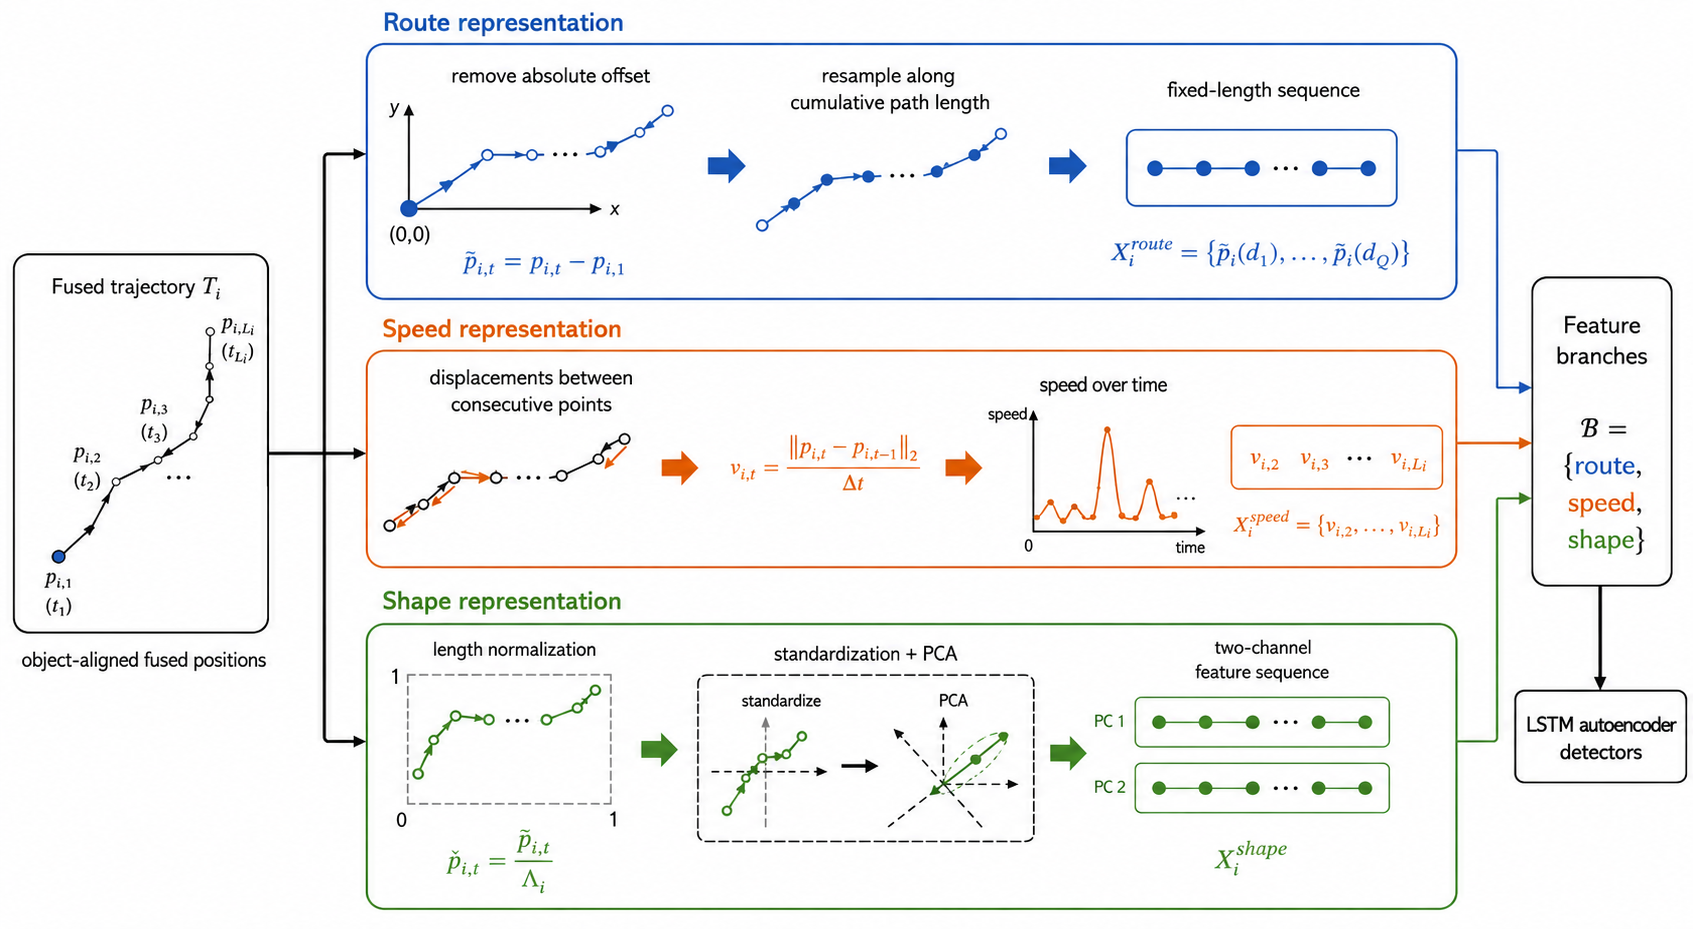
\includegraphics[width=\linewidth]{images/chapter5/route_speed_shape_feature_construction.png}
  \caption{Route, speed, and shape feature construction from a fused target trajectory. The fused trajectory is converted into a route sequence by removing the initial offset and resampling along cumulative distance, a speed sequence by frame-wise displacement over elapsed time, and a shape sequence by length normalization, standardization, and principal component projection.}
  \label{fig:chapter5-route-speed-shape-feature}
\end{figure}

\subsection{Route-Speed-Shape Feature Construction}
For a fused entity \(e_i\), let \((p_{i,t},\gamma_{i,t})\) denote the \(t\)-th observation extracted from the fused trajectory \(T_i\), where \(p_{i,t}=[x_{i,t},y_{i,t}]\), \(\gamma_{i,t}\) is the observation timestamp, and \(t=1,\ldots,L_i\). Feature construction is applied only when the number of valid observations and the path length exceed predefined thresholds used throughout the experiment. The numerical constant \(\epsilon\) is also fixed before testing. The first representation is the route feature, which describes the target's spatial path after removing the absolute starting position. Each point is converted into a relative coordinate
\begin{equation}
  \tilde{p}_{i,t} = p_{i,t} - p_{i,1}.
\end{equation}
The cumulative path length is then computed as
\begin{equation}
  d_{i,t}=\sum_{r=2}^{t}\left\|\tilde{p}_{i,r}-\tilde{p}_{i,r-1}\right\|_2,
\end{equation}
which gives the traveled distance from the starting point to the \(t\)-th observation. The relative trajectory is then resampled on this cumulative-distance axis to a fixed number of positions. Let \(d_q\), \(q=1,\ldots,Q\), denote uniformly selected distance values between the start and the end of the trajectory. The notation \(\tilde{p}_{i}(d_q)\) denotes the relative position obtained by linear interpolation at distance \(d_q\), rather than the position at a particular frame index. This produces a fixed-length route sequence
\begin{equation}
  X_{i}^{\mathrm{route}}=\{\tilde{p}_{i}(d_1),\tilde{p}_{i}(d_2),\ldots,\tilde{p}_{i}(d_Q)\}.
\end{equation}
Thus, fused trajectories with different frame numbers or sampling rates are converted into comparable route features. This representation emphasizes the path followed by the target and reduces sensitivity to the absolute coordinate offset between scenes.

The second representation is the speed feature. For consecutive observations in the fused trajectory, the scalar speed is estimated by
\begin{equation}
  u_{i,t}=
  \frac{\left\|p_{i,t}-p_{i,t-1}\right\|_2}
  {\max(\gamma_{i,t}-\gamma_{i,t-1},\epsilon)},
\end{equation}
where \(\epsilon\) is a small constant used to avoid numerical instability. The speed sequence is written as
\begin{equation}
  X_{i}^{\mathrm{speed}}=\{u_{i,2},u_{i,3},\ldots,u_{i,L_i}\}.
\end{equation}
Compared with the route representation, the speed representation is more sensitive to abrupt acceleration, abnormal stopping, and unusually fast movement.

The third representation is the shape feature. Shape is intended to describe the geometry of the motion rather than the absolute position or the total path length. Consecutive duplicate positions are removed first. If the remaining trajectory has a path length below the predefined threshold or is shorter than the minimum sequence length, the shape feature is treated as unavailable. Otherwise, the relative coordinates are normalized by the total path length
\begin{equation}
  \Lambda_i=\sum_{t=2}^{L_i}\left\|\tilde{p}_{i,t}-\tilde{p}_{i,t-1}\right\|_2,\qquad
  \breve{p}_{i,t}=\frac{\tilde{p}_{i,t}}{\Lambda_i}.
\end{equation}
The normalized curve is resampled along a normalized temporal axis and standardized using training-set statistics. The principal component projection is fitted on the training shape sequences only and then applied unchanged to validation and test trajectories. The resulting two-channel sequence is denoted as \(X_{i}^{\mathrm{shape}}\). The detector set therefore contains three fused-trajectory feature branches:
\begin{equation}
  \mathcal{B}=\{\mathrm{route},\mathrm{speed},\mathrm{shape}\}.
\end{equation}
The multimodal information enters this stage through the fused trajectory itself, so no separate RGB or thermal detector branch is introduced here.

\subsection{LSTM Autoencoder-Based Detector}
For each feature branch \(a\in\mathcal{B}\), all valid sequences are collected as \(\{X_i^{(a)}\}\), where \(X_i^{(a)}\in\mathbb{R}^{L_i^{(a)}\times d_a}\), \(L_i^{(a)}\) is the branch-specific sequence length, and \(d_a\) is the feature dimension. Before training, the sequence values are normalized using statistics estimated from the training split. Because different targets have different valid lengths, sequences are padded within each mini-batch and a binary mask \(M_i^{(a)}\) identifies valid time steps. The complete individual-level detection workflow is summarized in Figure~\ref{fig:chapter5-individual-anomaly-workflow}: branch-specific LSTM autoencoders provide reconstruction evidence, embedding-space neighborhoods adjust branch scores, and rank-based ensemble scoring produces the final individual anomaly score.

\begin{figure}[htbp]
  \centering
  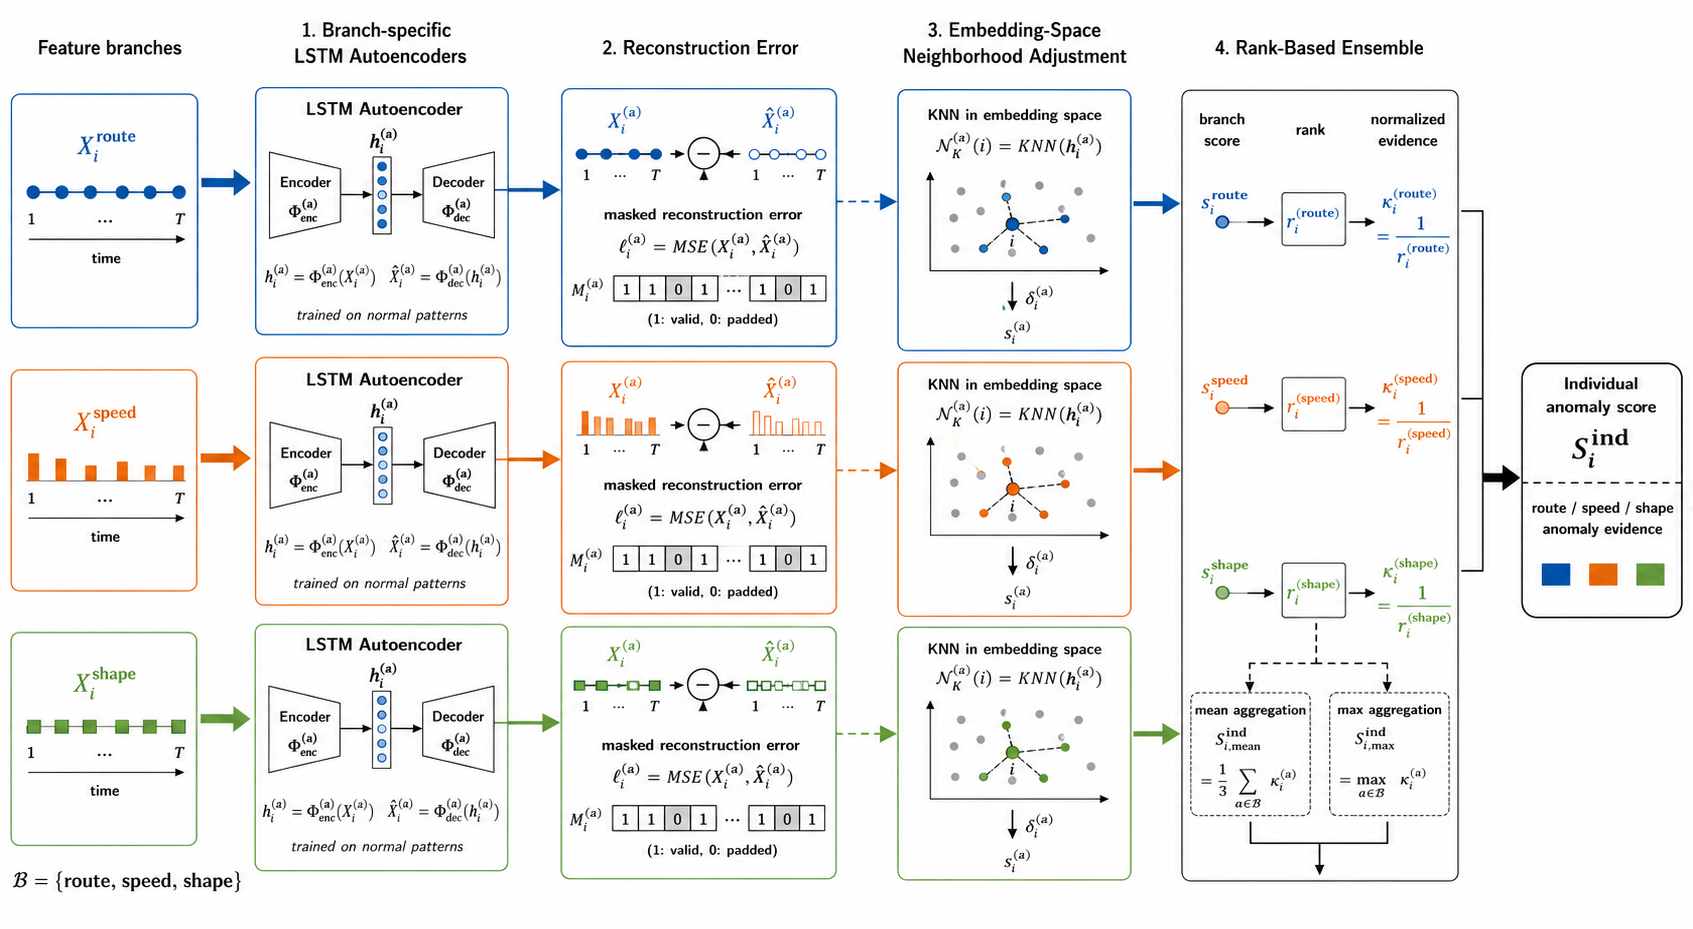
\includegraphics[width=\linewidth]{images/chapter5/individual_anomaly_detection_workflow.png}
  \caption{Individual-level anomaly detection workflow. Route, speed, and shape feature sequences are processed by branch-specific LSTM autoencoders. Masked reconstruction errors are adjusted by embedding-space neighborhoods, and branch-level scores are fused through rank-based ensemble scoring to obtain the individual anomaly score.}
  \label{fig:chapter5-individual-anomaly-workflow}
\end{figure}

Each branch is modeled by an LSTM autoencoder. The encoder maps a normalized feature sequence to a compact embedding:
\begin{equation}
  h_i^{(a)}=\Phi_{\mathrm{enc}}^{(a)}\big(X_i^{(a)}\big),
\end{equation}
where \(h_i^{(a)}\) is the latent representation of entity \(i\) under branch \(a\). The decoder repeats this latent vector along the temporal dimension and reconstructs the original sequence:
\begin{equation}
  \hat{X}_i^{(a)}=\Phi_{\mathrm{dec}}^{(a)}\big(h_i^{(a)},L_i^{(a)}\big).
\end{equation}
The model is trained to minimize the reconstruction error on valid, non-padded positions:
\begin{equation}
  \mathcal{L}^{(a)} =
  \frac{1}{|\mathcal{D}_{\mathrm{tr}}|}
  \sum_{i\in\mathcal{D}_{\mathrm{tr}}}
  \frac{
  \sum_{t=1}^{L_i^{(a)}} M_{i,t}^{(a)}
  \left\|X_{i,t}^{(a)}-\hat{X}_{i,t}^{(a)}\right\|_2^2
  }
  {
  d_a\sum_{t=1}^{L_i^{(a)}}M_{i,t}^{(a)}+\epsilon
  }.
\end{equation}
After training, the per-sample reconstruction error is used as the initial anomaly evidence:
\begin{equation}
  \ell_i^{(a)} =
  \frac{
  \sum_{t=1}^{L_i^{(a)}} M_{i,t}^{(a)}
  \left\|X_{i,t}^{(a)}-\hat{X}_{i,t}^{(a)}\right\|_2^2
  }
  {
  d_a\sum_{t=1}^{L_i^{(a)}}M_{i,t}^{(a)}+\epsilon
  }.
\end{equation}
A high value of \(\ell_i^{(a)}\) indicates that the corresponding route, speed, or shape sequence is difficult to reconstruct using the normal-pattern model.

\subsection{Neighborhood-Adjusted Anomaly Score}
Directly using reconstruction error may be unstable when some normal trajectory groups are intrinsically difficult to reconstruct. To reduce this effect, the detector adjusts the reconstruction error by comparing each trajectory with its nearest neighbors in the learned embedding space. For branch \(a\), the neighborhood of entity \(i\) is defined as
\begin{equation}
  \mathcal{N}_K^{(a)}(i)=
  \operatorname{KNN}
  \big(h_i^{(a)},
  \{h_j^{(a)}\mid j\in\mathcal{D}_{\mathrm{ref}}^{(a)}, j\neq i\},K\big),
\end{equation}
where \(K\) is the number of neighbors and \(\mathcal{D}_{\mathrm{ref}}^{(a)}\) denotes a fixed reference embedding set, such as the normal training set or a historical reference set. This prevents the neighborhood adjustment from depending on the composition of a test batch. The local loss deviation of entity \(i\) is then computed as
\begin{equation}
  \delta_i^{(a)}=
  \frac{1}{|\mathcal{N}_K^{(a)}(i)|}
  \sum_{j\in\mathcal{N}_K^{(a)}(i)}
  \left|\ell_i^{(a)}-\ell_j^{(a)}\right|.
\end{equation}
This term measures whether the reconstruction error of the target is unusual compared with trajectories that have similar latent motion patterns. The final branch-level anomaly score is normalized by the average local deviation of its neighbors:
\begin{equation}
  s_i^{(a)}=
  \frac{\delta_i^{(a)}}
  {
  \frac{1}{|\mathcal{N}_K^{(a)}(i)|}
  \sum_{j\in\mathcal{N}_K^{(a)}(i)}\delta_j^{(a)}+\epsilon
  }.
\end{equation}
If the neighborhood is too small or the denominator is numerically close to zero, the unnormalized local deviation is used as a fallback. In this way, a trajectory receives a high branch-level score only when its reconstruction behavior is locally inconsistent with similar trajectories, not merely when its raw reconstruction loss is large.

\subsection{Multi-Representation Detector Ensemble}
The above process produces one score vector for each valid branch \(a\in\mathcal{B}\). Because route, speed, and shape features have different validity requirements, the detector outputs are first aligned by fused entity identifier. If a branch does not produce a score for a target, for example because the fused trajectory is too short or its path length is below the predefined threshold, the missing value is filled with the median score of that branch. This keeps all valid fused entities in the ensemble while avoiding an overly strong missing-value penalty.

The scores from different branches are not directly comparable in scale, so the ensemble uses rank-based normalization. Let \(r_i^{(a)}\) denote the descending rank of \(s_i^{(a)}\) among all targets in branch \(a\), where a smaller rank means a more suspicious target. The normalized branch evidence is defined as
\begin{equation}
  \kappa_i^{(a)}=\frac{1}{r_i^{(a)}}.
\end{equation}
Two aggregate scores are then computed:
\begin{equation}
  S_{i,\mathrm{mean}}^{\mathrm{ind}}=
  \frac{1}{|\mathcal{B}|}\sum_{a\in\mathcal{B}}\kappa_i^{(a)},\qquad
  S_{i,\mathrm{max}}^{\mathrm{ind}}=
  \max_{a\in\mathcal{B}}\kappa_i^{(a)}.
\end{equation}
The mean score reflects consistent evidence across multiple representations, while the max score preserves strong complementary evidence from any single route, speed, or shape branch. The final individual-level anomaly score used in the fusion stage is defined as
\begin{equation}
  S_i^{\mathrm{ind}}=S_{i,\mathrm{mean}}^{\mathrm{ind}}.
\end{equation}
The max score \(S_{i,\mathrm{max}}^{\mathrm{ind}}\) is retained as a complementary diagnostic score for branch-specific anomalies. The implementation also records a complementary elimination process. At each iteration, one detector is removed and the change in the Top-\(K\) anomaly set is measured by Jaccard similarity. Detectors whose removal causes little change are considered redundant, and the resulting curve helps analyze the contribution of each feature branch.

\section{Group-Level Spatio-Temporal Graph Anomaly Detection}

The individual-level detector evaluates whether a fused trajectory is unusual by itself. Some abnormal behaviors, however, are relational. A target may leave a stable group, move against nearby targets, or appear in a group whose population changes suddenly. To keep this part simple and interpretable, this section uses a lightweight spatio-temporal graph to describe local group relations and computes group anomaly scores from graph-structure changes and group statistics. As summarized in Figure~\ref{fig:chapter5-lightweight-st-graph-events}, fused target states are first organized as target-frame nodes with spatial and temporal edges. Connected components are then tracked as groups, and interpretable object-to-group and group-level event indicators are fused into group anomaly scores. No manually labeled group anomaly categories are required.

\begin{figure}[htbp]
  \centering
  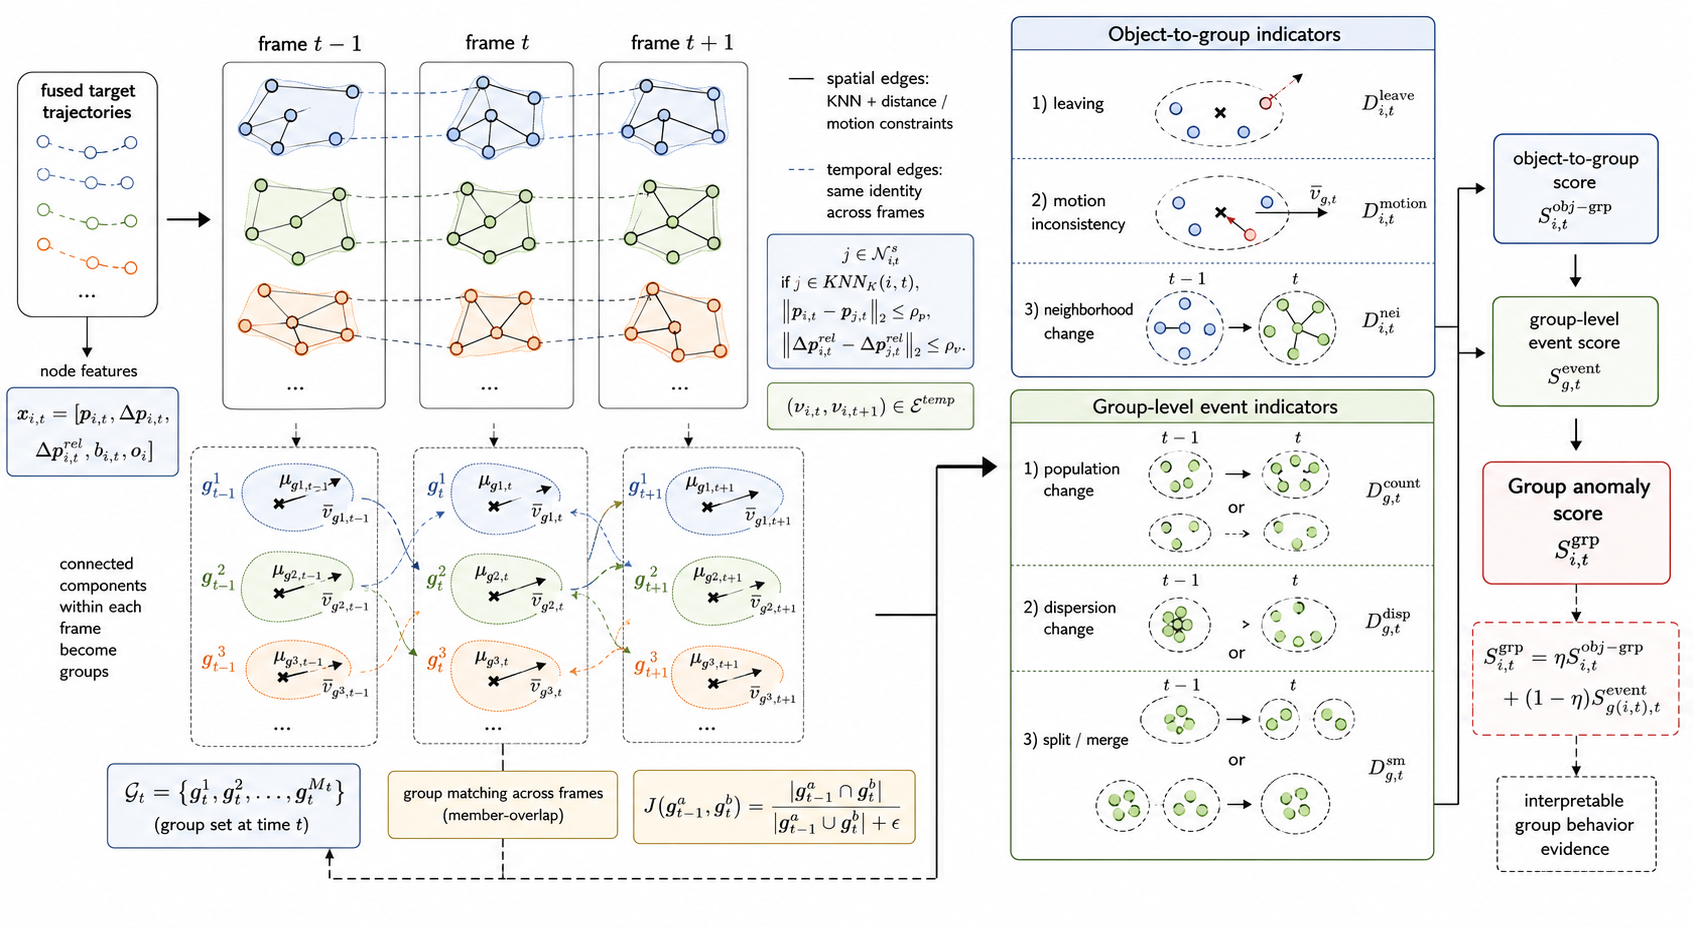
\includegraphics[width=\linewidth]{images/chapter5/lightweight_spatiotemporal_graph_group_events.png}
  \caption{Lightweight spatio-temporal graph and group event indicators. Fused target states are represented as target-frame nodes. Spatial edges describe local motion-consistent neighborhoods, and temporal edges preserve identity continuity. Connected components define candidate groups, while interpretable indicators describe object-to-group deviations and group-level events such as leaving, motion inconsistency, population change, dispersion change, split, and merge.}
  \label{fig:chapter5-lightweight-st-graph-events}
\end{figure}

\subsection{Spatio-Temporal Graph Construction}
For a sequence of frames, a sliding temporal window is defined as
\begin{equation}
  \mathcal{W}_t = \{t-L_{\mathrm{in}}+1,\ldots,t\},
\end{equation}
where \(L_{\mathrm{in}}\) is the input window length. Each visible fused target at each frame is represented as a target-frame node \(\nu_{i,\tau}\), where \(i\) denotes the target identity and \(\tau\in\mathcal{W}_t\). The node feature is constructed from the fused trajectory and basic target attributes:
\begin{equation}
  x_{i,\tau}=
  \big[p_{i,\tau},\,\Delta p_{i,\tau},\,\Delta p^{\mathrm{rel}}_{i,\tau},\,b_{i,\tau},\,o_i\big],
\end{equation}
where \(p_{i,\tau}\) is the fused target center, \(\Delta p_{i,\tau}=p_{i,\tau}-p_{i,\tau-1}\) is the target displacement, \(b_{i,\tau}\) denotes the bounding-box size, and \(o_i\) is the one-hot category vector. Because VT-Tiny-MOT is captured from aerial platforms, frame-level camera motion may cause many targets to move coherently in image coordinates. To reduce this effect, the relative displacement is defined as
\begin{equation}
  \Delta p^{\mathrm{rel}}_{i,\tau}
  =
  \Delta p_{i,\tau}
  -
  \mathrm{median}_{j\in\mathcal{V}_{\tau}}\big(\Delta p_{j,\tau}\big),
\end{equation}
where \(\mathcal{V}_{\tau}\) is the set of visible targets at frame \(\tau\). This term makes the graph focus on target motion relative to the local scene rather than on global image displacement.

The graph contains spatial edges and temporal edges. Spatial edges are constructed within each frame by a simple \(K\)-nearest-neighbor rule with distance and motion constraints:
\begin{equation}
  j\in\mathcal{N}_{i,\tau}^{s}
  \Longleftrightarrow
  j\in\operatorname{KNN}_{K}(i,\tau),\quad
  \|p_{i,\tau}-p_{j,\tau}\|_2\leq\rho_p,\quad
  \|\Delta p^{\mathrm{rel}}_{i,\tau}-\Delta p^{\mathrm{rel}}_{j,\tau}\|_2\leq\rho_v.
\end{equation}
Here \(\rho_p\) and \(\rho_v\) control the maximum spatial distance and relative-motion difference allowed for a local group relation. In implementation, \(p_{i,\tau}\) and \(\Delta p^{\mathrm{rel}}_{i,\tau}\) are measured in the unified plane provided by the fusion module. The parameters \(K\), \(\rho_p\), and \(\rho_v\) are fixed on the validation split and then kept unchanged for all test sequences. Temporal edges connect the same target across adjacent frames:
\begin{equation}
  \mathcal{E}^{\mathrm{temp}}=\{(\nu_{i,\tau},\nu_{i,\tau+1})\mid i \text{ is visible at both } \tau \text{ and } \tau+1\}.
\end{equation}
This graph is intentionally simpler than the relation-aware graph in Chapter 4. Chapter 4 uses graph reasoning for cross-modal entity fusion, whereas this chapter uses the graph to describe local behavior relations after fusion has been completed.

\subsection{Group Discovery and Event Indicators}
The spatial graph at each frame provides a direct basis for discovering target groups. Connected components in the spatial graph are treated as candidate groups:
\begin{equation}
  \mathcal{G}_{\tau}=\{g_{\tau}^{1},g_{\tau}^{2},\ldots,g_{\tau}^{M_{\tau}}\},
\end{equation}
where each group \(g_{\tau}^{m}\subseteq\mathcal{V}_{\tau}\) contains targets that are spatially close and motion-consistent at frame \(\tau\). Isolated targets are kept as single-target components, because isolation itself may be useful evidence for anomaly detection.

To describe group evolution across time, groups in adjacent frames are matched by member overlap. For two candidate groups \(g_{\tau-1}^{a}\) and \(g_{\tau}^{b}\), their temporal continuity score is
\begin{equation}
  J(g_{\tau-1}^{a},g_{\tau}^{b})
  =
  \frac{|g_{\tau-1}^{a}\cap g_{\tau}^{b}|}
  {|g_{\tau-1}^{a}\cup g_{\tau}^{b}|+\epsilon}.
\end{equation}
A temporal match is accepted when \(J(\cdot)\) is greater than the overlap threshold \(\theta_J\), which is fixed before testing. If a group in frame \(\tau\) has one accepted predecessor, it is considered a continuation of the previous group and inherits its propagated group identity. If one previous group corresponds to multiple current groups, a split event is recorded. If multiple previous groups correspond to one current group, a merge event is recorded. If a group has no reliable predecessor or successor, it is interpreted as group appearance or disappearance.

For each group \(g_{\tau}\), several interpretable group statistics are computed:
\begin{equation}
  n_{g,\tau}=|g_{\tau}|,\qquad
  \mu_{g,\tau}=\frac{1}{n_{g,\tau}}\sum_{i\in g_{\tau}}p_{i,\tau},
\end{equation}
\begin{equation}
  \delta_{g,\tau}=
  \frac{1}{n_{g,\tau}}\sum_{i\in g_{\tau}}\|p_{i,\tau}-\mu_{g,\tau}\|_2,
  \qquad
  \bar{v}_{g,\tau}=
  \frac{1}{n_{g,\tau}}\sum_{i\in g_{\tau}}\Delta p^{\mathrm{rel}}_{i,\tau}.
\end{equation}
Here \(n_{g,\tau}\) measures group size, \(\mu_{g,\tau}\) is the group center, \(\delta_{g,\tau}\) describes group dispersion, and \(\bar{v}_{g,\tau}\) describes group-level motion. These statistics provide interpretable evidence for distinguishing whether an anomaly is caused by an individual leaving the group, a group changing its population, or a structural event such as splitting or merging.

\subsection{Interpretable Group Anomaly Score}
The group detector converts the above graph statistics into a small set of interpretable anomaly scores. Let \(g(i,t)\) be the group containing target \(i\) at frame \(t\). The group-leaving score is defined as
\begin{equation}
  D_{i,t}^{\mathrm{leave}}
  =
  \left[
  \frac{
  \|p_{i,t}-\mu_{g(i,t),t}\|_2
  -
  \mathrm{median}_{\tau\in[t-W,t-1]}
  \|p_{i,\tau}-\mu_{g(i,\tau),\tau}\|_2
  }
  {
  \mathrm{MAD}_{\tau\in[t-W,t-1]}
  \|p_{i,\tau}-\mu_{g(i,\tau),\tau}\|_2+\epsilon
  }
  \right]_{+},
\end{equation}
where \([\cdot]_+=\max(\cdot,0)\). This score becomes high when a target moves farther away from its historical group center. The motion-inconsistency score is
\begin{equation}
  D_{i,t}^{\mathrm{motion}}
  =
  1-
  \frac{
  \langle \Delta p^{\mathrm{rel}}_{i,t},\bar{v}_{g(i,t),t}\rangle
  }
  {
  \|\Delta p^{\mathrm{rel}}_{i,t}\|_2\|\bar{v}_{g(i,t),t}\|_2+\epsilon
  },
\end{equation}
which detects targets moving against or away from the group direction. The neighborhood-change score is
\begin{equation}
  D_{i,t}^{\mathrm{nei}}
  =
  1-
  \frac{
  |\mathcal{N}_{i,t}^{s}\cap\mathcal{N}_{i,t-1}^{s}|
  }
  {
  |\mathcal{N}_{i,t}^{s}\cup\mathcal{N}_{i,t-1}^{s}|+\epsilon
  }.
\end{equation}
This term captures sudden neighbor replacement, which may correspond to leaving, entering, crossing, or merging with a group.

Group-level event deviation is measured for tracked groups whose identities are propagated through the overlap-based matching rule. For a tracked group \(g\), the population-change score is
\begin{equation}
  D_{g,t}^{\mathrm{count}}
  =
  \frac{
  |n_{g,t}-\mathrm{median}_{\tau\in[t-W,t-1]}n_{g,\tau}|
  }
  {
  \mathrm{MAD}_{\tau\in[t-W,t-1]}n_{g,\tau}+\epsilon
  },
\end{equation}
where the historical terms are computed only over frames in which the same propagated group identity is available. The dispersion-change score is
\begin{equation}
  D_{g,t}^{\mathrm{disp}}
  =
  \frac{
  |\delta_{g,t}-\mathrm{median}_{\tau\in[t-W,t-1]}\delta_{g,\tau}|
  }
  {
  \mathrm{MAD}_{\tau\in[t-W,t-1]}\delta_{g,\tau}+\epsilon
  }.
\end{equation}
The split-or-merge indicator is defined according to the same group matching results:
\begin{equation}
  D_{g,t}^{\mathrm{sm}}=
  \mathbb{I}(g \text{ is involved in a split or merge event}).
\end{equation}
These terms describe whether a group suddenly gains or loses members, becomes unusually compact or dispersed, or undergoes structural reorganization.

All component scores are robustly normalized by the median and median absolute deviation computed on the training set. Let \(\mathcal{R}(\cdot)\) denote this normalization. The weights \(\alpha_1,\alpha_2,\alpha_3,\beta_1,\beta_2,\beta_3\) are non-negative, and \(\eta\in[0,1]\). These parameters are fixed on the validation split and are not adjusted for individual test sequences. The object-to-group anomaly score is
\begin{equation}
  S_{i,t}^{\mathrm{obj\mbox{-}grp}}
  =
  \alpha_1\mathcal{R}(D_{i,t}^{\mathrm{leave}})
  +
  \alpha_2\mathcal{R}(D_{i,t}^{\mathrm{motion}})
  +
  \alpha_3\mathcal{R}(D_{i,t}^{\mathrm{nei}}).
\end{equation}
The group-event anomaly score is
\begin{equation}
  S_{g,t}^{\mathrm{event}}
  =
  \beta_1\mathcal{R}(D_{g,t}^{\mathrm{count}})
  +
  \beta_2\mathcal{R}(D_{g,t}^{\mathrm{disp}})
  +
  \beta_3D_{g,t}^{\mathrm{sm}}.
\end{equation}
Finally, the frame-level group anomaly score of target \(i\) is
\begin{equation}
  S_{i,t}^{\mathrm{grp}}
  =
  \eta S_{i,t}^{\mathrm{obj\mbox{-}grp}}
  +
  (1-\eta)S_{g(i,t),t}^{\mathrm{event}},
\end{equation}
and the object-level group anomaly score is obtained by a high-percentile aggregation:
\begin{equation}
  S_{i}^{\mathrm{grp}}
  =
  \operatorname{Percentile}_{95}
  \left(\{S_{i,t}^{\mathrm{grp}}\}_{t=1}^{L_i}\right).
\end{equation}
The dominant anomaly reason is determined by the largest normalized component in the score decomposition. For instance, a high \(D^{\mathrm{leave}}\) indicates group leaving, a high \(D^{\mathrm{nei}}\) indicates neighborhood restructuring, a high \(D^{\mathrm{count}}\) indicates sudden population change, and \(D^{\mathrm{sm}}\) directly indicates a split or merge event. Therefore, the group detector does not only output a scalar anomaly score, but also provides interpretable evidence for the type of group-level abnormal behavior.

\section{Individual-Group Fusion and Situation Output}

\subsection{Individual-Group Score Fusion}
The individual-level detector and the group-level detector describe different abnormality sources. The individual score \(S_i^{\mathrm{ind}}\) focuses on the target trajectory itself, while the group score \(S_i^{\mathrm{grp}}\) focuses on whether the target is consistent with its surrounding group and whether the group undergoes abnormal structural evolution. These two scores are therefore complementary rather than mutually exclusive. Before fusion, both scores are transformed to a comparable scale by robust normalization:
\begin{equation}
  \tilde{S}_i^{\mathrm{ind}}
  =
  \mathcal{R}\big(S_i^{\mathrm{ind}}\big),\qquad
  \tilde{S}_i^{\mathrm{grp}}
  =
  \mathcal{R}\big(S_i^{\mathrm{grp}}\big),
\end{equation}
where \(\mathcal{R}(\cdot)\) denotes median-and-MAD normalization estimated from the training split. The fused object-level anomaly score is then defined as
\begin{equation}
  S_i^{\mathrm{fuse}}
  =
  \alpha \tilde{S}_i^{\mathrm{ind}}
  +
  (1-\alpha)\tilde{S}_i^{\mathrm{grp}},
\end{equation}
where \(\alpha\in[0,1]\) controls the relative contribution of individual and group evidence. The fusion weight is selected on the validation split and is not adjusted separately for individual test sequences. When only an individual score is available, the fused score falls back to \(\tilde{S}_i^{\mathrm{ind}}\); when only a group score is available, it falls back to \(\tilde{S}_i^{\mathrm{grp}}\). This fallback design is necessary because some targets may be too short for all individual feature branches, while some frames may contain too few neighboring targets for reliable group modeling.

In addition to the scalar fused score, the fusion stage preserves the component scores:
\begin{equation}
  S_i^{\mathrm{obj\mbox{-}grp}}
  =
  \operatorname{Percentile}_{95}
  \left(\{S_{i,t}^{\mathrm{obj\mbox{-}grp}}\}_{t=1}^{L_i}\right),
  \qquad
  S_i^{\mathrm{event}}
  =
  \operatorname{Percentile}_{95}
  \left(\{S_{g(i,t),t}^{\mathrm{event}}\}_{t=1}^{L_i}\right),
\end{equation}
\begin{equation}
  \Omega_i=
  \{S_i^{\mathrm{ind}},S_i^{\mathrm{grp}},
  S_i^{\mathrm{obj\mbox{-}grp}},S_i^{\mathrm{event}}\}.
\end{equation}
The component record makes the final output interpretable. If \(S_i^{\mathrm{ind}}\) dominates, the abnormality is mainly caused by the target's own route, speed, or shape. If \(S_i^{\mathrm{obj\mbox{-}grp}}\) dominates, the abnormality is mainly a target-to-group deviation such as leaving, entering, or moving against the local group. If \(S_i^{\mathrm{event}}\) dominates, the abnormality is mainly caused by a group event such as population change, split, merge, or dispersion change.

\subsection{Anomaly Event Decision}
The fused score can fluctuate at a single frame because of detection noise, temporary occlusion, or short-term tracking instability. Therefore, event decisions are made after temporal smoothing. Let \(S_{i,t}^{\mathrm{fuse}}\) denote the frame-level fused score before target-level aggregation. A smoothed score is computed by an exponential moving average:
\begin{equation}
  \bar{S}_{i,t}^{\mathrm{fuse}}
  =
  \lambda_s\bar{S}_{i,t-1}^{\mathrm{fuse}}
  +
  (1-\lambda_s)S_{i,t}^{\mathrm{fuse}},
\end{equation}
where \(\lambda_s\in[0,1]\) controls the smoothing strength. The anomaly event decision is then defined as
\begin{equation}
  y_{i,t}
  =
  \mathbb{I}\left(
  \bar{S}_{i,t}^{\mathrm{fuse}}>\theta
  \right),
\end{equation}
where \(\theta\) is selected according to the desired false alarm level or by a fixed top-percentile rule on the validation split. The smoothing factor \(\lambda_s\) and the decision threshold \(\theta\) are fixed before testing. To avoid reporting many fragmented alarms for the same target, consecutive abnormal frames are merged into one event segment:
\begin{equation}
  \mathcal{I}_i^{\mathrm{evt}} =
  \{[t_s,t_e]\mid y_{i,t}=1,\ t_s\leq t\leq t_e\}.
\end{equation}
Each event segment is assigned an event score by the maximum or high-percentile value within the segment:
\begin{equation}
  S([t_s,t_e])
  =
  \operatorname{Percentile}_{95}
  \left(
  \{\bar{S}_{i,t}^{\mathrm{fuse}}\mid t\in[t_s,t_e]\}
  \right).
\end{equation}
The event type is determined from the largest component score inside the segment. This yields interpretable labels such as route anomaly, speed anomaly, shape anomaly, group leaving, motion inconsistency, neighborhood restructuring, population change, split, and merge.

\subsection{Situation Heatmap Generation}
The final output of behavior analysis should support situation interpretation rather than only provide object-level rankings. For this purpose, object-level anomaly evidence is projected back to the image plane or the unified spatial plane and accumulated into a regional situation heatmap. For frame \(t\), the heatmap value at location \((x,y)\) is defined as
\begin{equation}
  \Xi_t(x,y)
  =
  \sum_{i\in\mathcal{V}_t}
  \bar{S}_{i,t}^{\mathrm{fuse}}
  K_{\sigma}
  \big((x,y)-p_{i,t}\big),
\end{equation}
where \(K_{\sigma}(\cdot)\) is a Gaussian kernel with bandwidth \(\sigma\). The bandwidth is fixed for all sequences. This formulation differs from a conventional target-density map because each target is weighted by its anomaly score. Regions containing many normal targets do not necessarily become high-risk regions, while a small number of highly abnormal targets can still create a visible hotspot.

For temporal situation analysis, frame-level heatmaps can be accumulated with a decay factor:
\begin{equation}
  \bar{\Xi}_t(x,y)
  =
  \lambda_h\bar{\Xi}_{t-1}(x,y)
  +
  (1-\lambda_h)\Xi_t(x,y),
\end{equation}
where \(\lambda_h\) controls how long recent anomaly evidence remains visible and is fixed before testing. The regional situation intensity of a spatial cell \(\mathcal{P}\) is then
\begin{equation}
  I_t(\mathcal{P})
  =
  \frac{1}{|\mathcal{P}|}
  \int_{(x,y)\in\mathcal{P}}
  \bar{\Xi}_t(x,y)\,dx\,dy.
\end{equation}
This output connects object-level anomaly detection with situation-level visualization. It allows the system to identify not only which target is abnormal, but also where abnormal behavior is concentrated and how the regional risk changes over time.

\section{Experiments and Result Analysis}

\subsection{Dataset and Experimental Setting}
The experiment in this chapter uses the VT-Tiny-MOT dataset. VT-Tiny-MOT is a visible-infrared multi-object tracking dataset collected from aerial scenes. Each sequence contains paired image streams and target annotations, which makes it suitable for constructing object-centered trajectories and demonstrating downstream behavior analysis from fused target representations. The image sequences also cover different scene layouts, target densities, illumination conditions, and motion patterns. They therefore provide a practical input source for examining the visualization stage of the proposed anomaly detection framework.

This dataset is used here for two reasons. First, its tracking-oriented annotations are consistent with the input form required by this chapter: the behavior detector operates on fused trajectories rather than on isolated video frames. Second, the dataset contains multiple real aerial scenes, which makes the generated heatmaps easier to interpret at the situation level. However, VT-Tiny-MOT does not provide manually annotated individual or group anomaly labels. Therefore, the experiment in this chapter is organized as a qualitative visualization study rather than a supervised detection benchmark. Precision, recall, average precision, and other label-dependent metrics are not reported. The results are used only to examine whether object-aligned anomaly scores can be projected into interpretable scene-level heatmaps.

The test output contains ten video sequences. For each sequence, the final result is presented as an anomaly heatmap overlaid on the original scene. The heatmap is not a target-density map or a manual abnormal-region annotation. Each target point contributes to nearby spatial regions according to its anomaly score, so a high-value region means that model-derived anomaly evidence is spatially concentrated there.

\subsection{Qualitative Heatmap Results}
Figure~\ref{fig:chapter5-heatmap-examples} compares the original frames and the corresponding anomaly heatmaps for the ten test sequences used in this chapter. The upper row shows the original aerial frames, and the lower row overlays score-weighted anomaly evidence on the same scenes. Bright regions indicate where model-derived anomaly evidence is accumulated after spatial projection. In sequences with a concentrated response, the heatmap highlights a local road, waterway, or scene region where high-scoring trajectory points appear repeatedly. In sequences with a weaker or more dispersed response, the heatmap remains mostly low-valued, indicating that no dominant spatial hotspot is formed.

\begin{figure}[H]
  \centering
  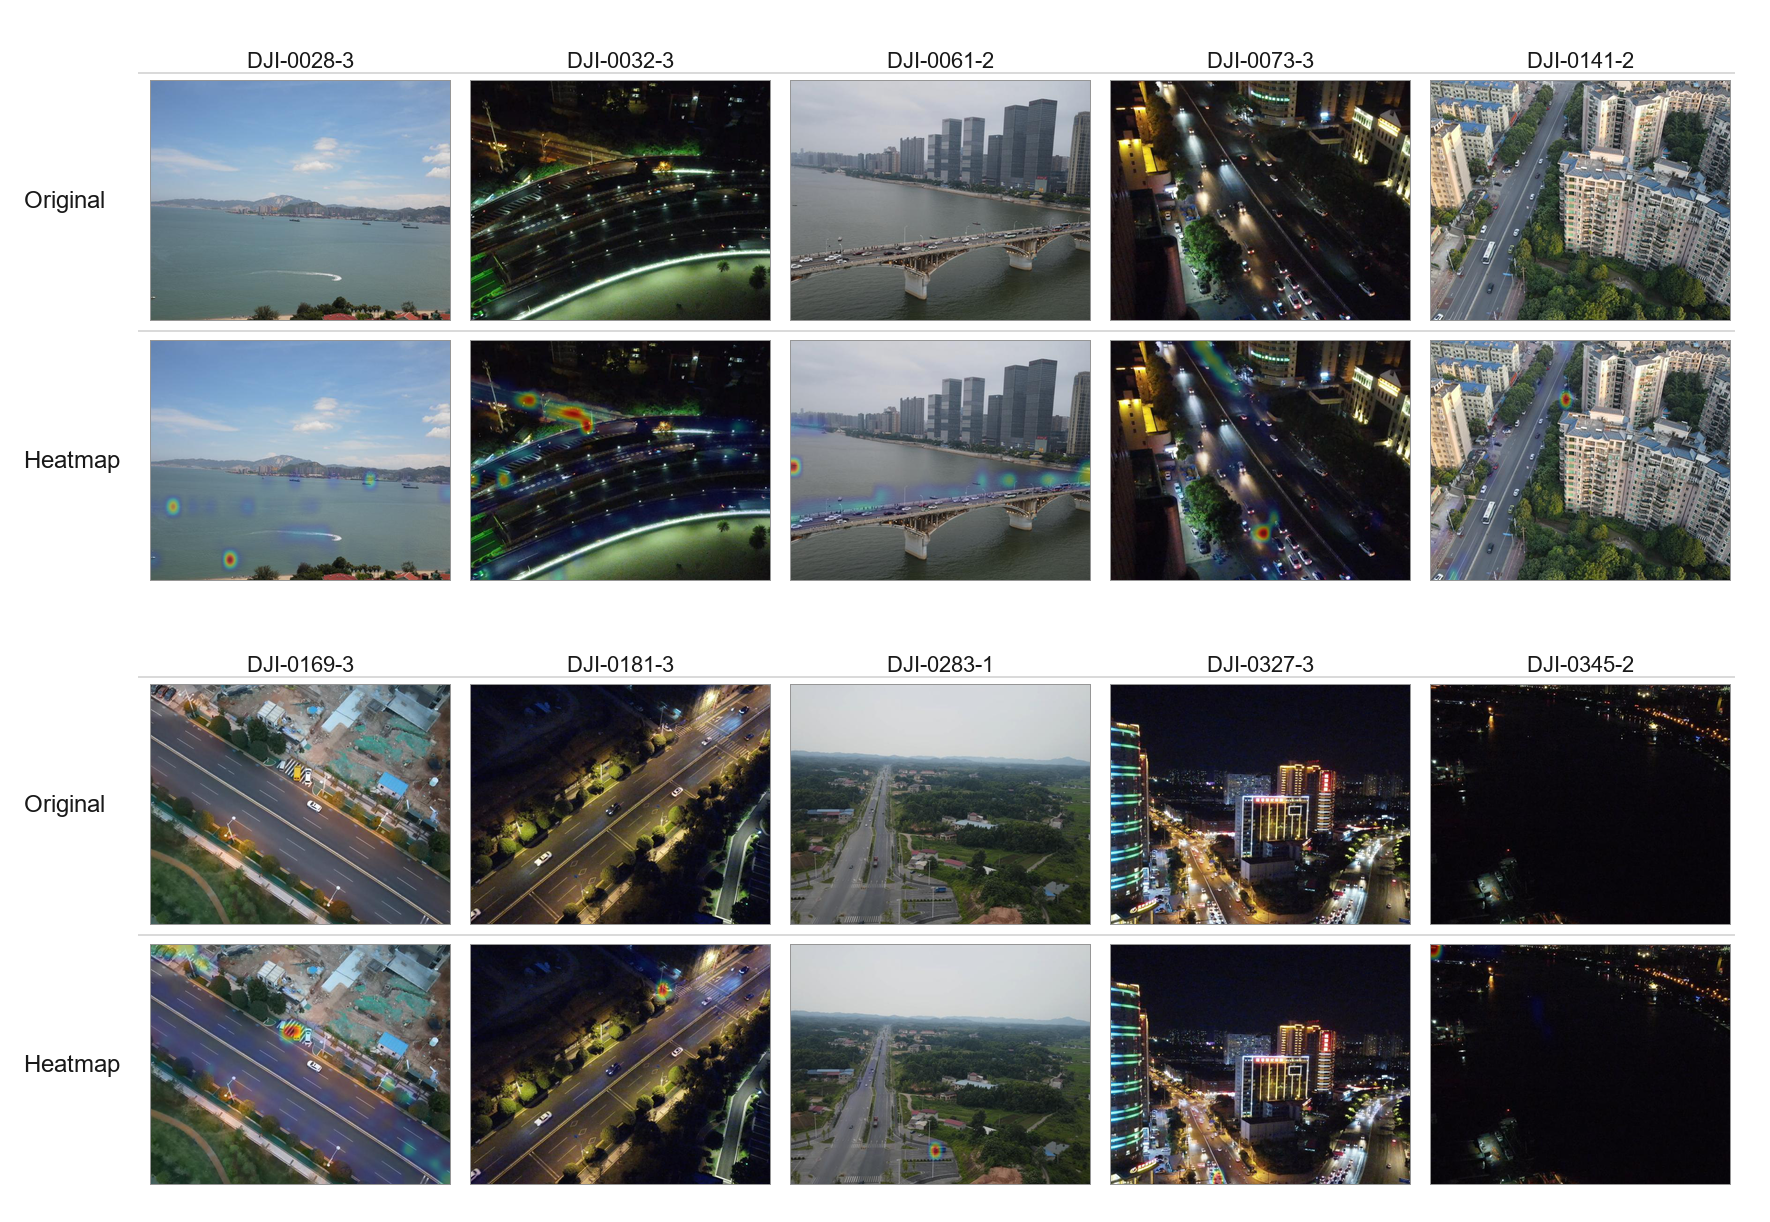
\includegraphics[width=0.88\linewidth]{images/chapter5/vt_tiny_mot_heatmap_overview.png}
  \caption{Original frames and anomaly heatmaps for the VT-Tiny-MOT test sequences. Each group contains five sequences. Within each group, the upper row shows the original frames, and the lower row shows the corresponding score-weighted heatmap visualization. The heatmaps visualize model-derived anomaly evidence rather than manually annotated abnormal regions.}
  \label{fig:chapter5-heatmap-examples}
\end{figure}

Across the ten test sequences, the heatmaps localize high-scoring trajectory evidence to specific scene regions when such evidence is spatially concentrated. Sequences with weaker or scattered scores produce diffuse low-intensity maps. These observations are consistent with the intended role of the heatmap as a scene-level visualization of object-aligned anomaly evidence.

\subsection{Discussion}
Because the current VT-Tiny-MOT output does not include manually verified anomaly labels, the experiment should be interpreted as a functional and qualitative demonstration rather than a quantitative detection benchmark. The experiment shows that fused trajectory-level anomaly evidence can be projected into spatial situation indicators, but it does not establish detection accuracy. A more complete evaluation would require frame-level or event-level anomaly annotations, which would make it possible to compare individual-only, group-only, and fused settings quantitatively.

\section{Chapter Summary}
This chapter developed a behavior anomaly detection framework based on the fused multimodal entities generated in Chapter 4. The task was defined as estimating individual and group anomaly evidence from fused trajectories, integrating them into object-level anomaly decisions, and projecting the results into regional situation indicators.

At the individual level, the method decomposes fused trajectories into route, speed, and shape representations. Masked LSTM autoencoders learn normal patterns, neighborhood-adjusted reconstruction errors produce branch-level scores, and rank-based ensemble scoring yields the final individual anomaly score.

At the group level, the chapter constructed a lightweight spatio-temporal graph in which target-frame nodes are linked by spatial group relations and temporal track continuity. Simple graph statistics describe interpretable events such as leaving, motion inconsistency, population change, split, and merge. Individual and group evidence are finally fused into anomaly-event scores and situation heatmaps. Under the qualitative evaluation setting used in this chapter, these outputs provide object-level anomaly cues and scene-level interpretation.
